% !TEX root = ../main.tex

\section{Introductory Remarks}

For better or worse, blockchain technologies like Ethereum have dramatically lowered the barrier to entry for developing and deploying financial technology. New tokens have been launched with a few clicks of a user interface, and large investment infrastructures have been developed and deployed with little regulatory oversight. Blockchain exchange services allow order-based trading of digital currencies, tokens, and other digital assets. Such exchanges are a key component to blockchain-based economic activity. 

For years, exchanges have operated either entirely off-chain by trusted operators or partially on-chain by semi-trusted operators. A fully on-chain exchange is feasible but considered too slow, at least for a public blockchain like Ethereum. We believe it is a very good time to do a deep dive into understanding precisely \textit{how slow} for the following reasons: (1) public blockchains are becoming faster (both in theory and slowly in practice) and the efficiency of an on-chain exchange will increase in time, (2) demand for on-chain trading is exemplified by the recent popularity of dealer-based (or quote-based) trading like Uniswap and Curve Finance, and (3) stablecoins have become popular and allow on-chain trading with pricing in USD (or other government currency).

\paragraph{Contributions.} We design and implement \cm, a fully on-chain call market in Solidity---a high-level programming language for Ethereum. We choose Ethereum as a `hostile' environment for an order book: Ethereum is public (strongest adversary) and slow (lower-bound benchmark) relative to more scalable blockchains, including the anticipated Ethereum 2.0. \cm is intended as a simple module that developers can modify as they choose. By adding \cm to an ERC20 (or similar) token contract, everything that is needed for buying/selling tokens is immediately available on chain without involving any third party exchanges. \cm is non-custodial, transparent, and mitigates front-running attacks that are generally possible on-chain.

While Solidity and EVM are like many common programming languages, they also have quirks that require experimentation to best optimize performance (\eg factoring in the gas costs of operations, gas refunds, limits to Solidity's object oriented design, clearing mappings). We test five priority queues---the core data structure of the call market---and various options for cleaning up our data once finished with it. The bottom line is that the current benchmark for a \cm-esque design is in the low hundreds of trade executions per block on Ethereum today. This positions \cm as a feasible design for certain types of markets today (low liquidity, small number of traders) but also as an early study on technology that is likely to improve vastly in the coming years. 

% = = = = = = = = = = = = = = = = = = = = = = = = = = = = = = = = = = = = = = = = = =
% = = = = = = = = = = = = = = = = = = = = = = = = = = = = = = = = = = = = = = = = = =
% = = = = = = = = = = = = = = = = = = = = = = = = = = = = = = = = = = = = = = = = = =

\section{Preliminaries}

\subsection{Market Structure}

\paragraph{Execution systems.} There are three main approaches to arranging a trade~\cite{Har03}. In a \emph{quote-driven} market, a dealer uses their own inventory to offer a price for buying or selling an asset. In a \emph{brokered exchange}, a broker finds a buyer and seller. In an \emph{order-driven} market, offers to buy (\emph{bids}) and sell (\emph{offers}/\emph{asks}) from many traders are placed as orders in an order book. Order-driven markets can be \emph{continuous}, with buyers/sellers at any time adding orders to the order book (\emph{makers}) or executing against an existing order (\emph{takers}); or they can be \emph{called}, where all traders submit orders within a window of time and orders are matched in a batch like an auction. 

\subsection{Decentralized Order Matching}

\paragraph{Central Exchanges (CEX).} Traditional financial markets (\eg NYSE and NASDAQ) use order-matching systems to arrange trades. An exchange will list one or more assets (stocks, bonds, derivatives, or more exotic securities) to be traded with each given its own order book priced in a currency (\eg USD). Exchanges for blockchain-based assets (also called crypto assets by enthusiasts) can operate the same way, using a centralized exchange (CEX) design where a firm operates the platform as a trusted third party in every aspect: custodianship over assets/currency being traded, exchanging assets fairly, and offering the best possible price execution. Security breaches and fraud (\eg MtGox~\cite{TheHisto45:online}, QuadrigaCX~\cite{SEBIOrde83:online}, and many others) in centralized exchanges have become a common source of lost funds for users, while accusations of unfair trade execution have been levelled but are difficult to prove. 

\paragraph{On-chain Order Books.} For trades between two blockchain-based assets (\eg a digital asset priced with a cryptocurrency, stablecoin, or second digital asset), order matching can be performed `on-chain' by deploying the order-matching system either on a dedicated blockchain or inside a decentralized application (DApp; \textit{a.k.a.} smart contract). In this model, traders entrust their assets to an autonomously operating DApp with known source code instead of a third party custodian that can abscond with or lose the funds. The trading rules will operate as coded, clearing and settling can be guaranteed, and order submission is handled by the blockchain---a reasonably fair and transparent system (but see front-running below). Finally, anyone can create an on-chain order book for any asset (on the same chain) at any time. While they sound ideal, performance is a substantial issue and the main subject of this paper. 

In this paper, we focus on benchmarking an order book for a public blockchain (\eg Ethereum). Ethereum is widely-used and we stand to learn the most from working in a performance-hostile environment (\ie Ethereum is good lower-bound). Exchanges could be given their own dedicated blockchain, where trade execution logic can be moved at the consensus level. Permissioned blockchains (\eg NASDAQ Linq, tZero) can also increase execution time and throughput, possibly with some reduction in transparency and trust.

\paragraph{On-chain Dealers.} Another on-chain advantage is that other smart contracts, not just human users, can initiate trades, enabling broader decentralized finance (DeFi) applications. This has fuelled a resurgence in on-chain exchange but through a quote-driven design rather than an order-driven one. Automated market makers  (\eg Uniswap) have all the trust advantages of an on-chain order book, plus they are very efficient relative to an on-chain order book. The trade-off is that they operate as a dealer---the DApp exchanges assets from its own inventory. This inventory is loaded into the DApp by an investor who will not make money on the trades themselves, but hope for long term profit through trading fees. By contrast, an order book requires no upfront inventory and does not have to charge trading fees (but can). Finally, there is a complicated difference in their price dynamics (\eg market impact of a trade, slippage between the best bid/ask and actual average execution price, \etc)---deserving of an entire research paper to precisely define. We leave it as an assertion that with equal liquidity, order books have more favourable price dynamics for traders.

\paragraph{Hybrid Designs.} Before on-chain dealers became prominent in the late 2010s, the most popular design was hybrid order-driven exchanges with some trusted off-chain components and some on-chain functionality. Some (\eg EtherDelta) were envisioned as operating fully on-chain, but performance limitations drove developers to move key components, such as the order matching system, off-chain to a centralized database. A landscape of DEX designs exist: many avoiding taking custodianship of assets off-chain, and virtually all (for order-driven markets) operate the order book itself off-chain. A non-custodial DEX solves the big issue of a CEX---the operator stealing the funds---however trade execution is still not provably fair. A mitigation is to issue a proof of correct execution to the DApp (\eg Loopring) but these proofs have blindspots (discussed in section~\ref{sec:rollups}). \cm offers key advantages in this model as well. 

\subsection{Related Works}

\paragraph{Blockchain Limitations and Solution.} While an order book is a ledger and blockchains provide a distributed ledger, it is not straightforward to drop a continuous-time order book onto a blockchain. An older 2014 paper~\cite{clark2014decentralizing} on the `Princeton prediction market'~\cite{Bra13} motivates our work. The authors observe the following limitations of on-chain continuous order books: block intervals are slow and not continuous, there is no support for accurate time-stamping, transactions can be dropped or reordered by miners, fast traders can react to submitted orders/cancelations when broadcast to network but not in a block and have their orders appear first (as examined in later work on front-running: \cite{eskandari2019sok,daian2019flash}).

\paragraph{Call Markets.} The researchers propose using a call market instead of a continuous-time market~\cite{clark2014decentralizing}. Orders are collected and placed into the order book over a window of time (\eg 1 or more blocks), then the market is closed and the orders are processed in batch: the best bids are matched to the best asks in order. If the prices overlap, the miner keeps the difference (which they could extract anyways through front-running). Call markets largely side-step front-running attacks from other traders because reordering trades has no impact (discussed more in section~\ref{sec:front}). The paper does not include an implementation and was envisioned as an alt-coin (Ethereum was still in development in 2014) with market closing being done by the miners themselves as part of the blockchain logic.

Large exchanges, like the NYSE and NASDAQ, use a two minute call market every day at opening and closing time (in between, the exchange runs as a continuous time market). Other exchanges, called crossing networks, also operate as a call market at various times throughout the trading day.\footnote{A crossing network uses a secondary market for determining the closing price. Many prominent crossing networks are operated internally within a brokerage for its clients, and often as a `	dark pool' with an unpublished order book.} Call market are studied widely in finance~\cite{Har03}. Time-sensitive traders submit orders early, especially in crossing networks that close at a randomly determined time (traders risk missing the call if they wait too long). A blockchain happens to provide this function naturally, as blocks are published unpredictably. Price-sensitive traders wait to base their pricing off the already submitted orders and do not mind missing a call if it obtains them a better price. 

\paragraph{Other Academic Literature.} There are numerous industry projects on blockchain-based exchanges and order books but most of the academic literature is on topics that are related but tangential to the mechanics of trade execution. Early literature considered trade execution under encryption (\ie dark markets)~\cite{TP07,YSLT10,TW12}. A number of projects consider structuring futures and derivatives in smart contracts---Velocity ~\cite{eskandari2017feasibility}, Findel ~\cite{biryukov2017findel}, FuturesMex~\cite{massacci2018futuresmex}---but once issued, the derivative can be traded using exchanges. Atomic swaps (\ie payment vs delivery) are necessary for settling trades and some general approaches include Arwen~\cite{heilman2020arwen} and Tesseract~\cite{bentov2017tesseract}.

% = = = = = = = = = = = = = = = = = = = = = = = = = = = = = = = = = = = = = = = = = =
% = = = = = = = = = = = = = = = = = = = = = = = = = = = = = = = = = = = = = = = = = =
% = = = = = = = = = = = = = = = = = = = = = = = = = = = = = = = = = = = = = = = = = =

\section{Priority Queues}\label{sec:pq}

% = = = = = = = = = = = =Operations for a generic Priority Queue Table = = =  = = = = = = = = = = = %
\begin{table}[t]
\setlength{\tabcolsep}{0.01\tabcolsep}% Shrink \tabcolsep
\centering
\begin{tabular}{|c|c|}
\hline

\textbf{Operation}   & \textbf{Description}    \\ \hline

% = = = = = = = = = = = = = = = = = = = = = = = = = = = = = = = = = = = = = = = = = = = = = = = = %
	\textbf{Enqueue()}       	& Inserts an element into the priority queue                        \\ \hline
	\textbf{Dequeue()}		& Removes and returns the highest priority element 		\\ \hline
	\textbf{isEmpty()}			& Checks if the priority queue is empty 					\\ \hline
% = = = = = = = = = = = = = = = = = = = = = = = = = = = = = = = = = = = = = = = = = = = = = = = =  %

\end{tabular}
\caption{\footnotesize{Operations for a generic priority queue.}
\label{tab:PQ_API}}
\end{table}
% = = = = = = = = = = = = = = = = = = = = =  = = = = = = = = = = =  = = = = = = = = = == = = =  = =%

In designing \cm within Ethereum's gas model, performance is the main bottleneck. For a call market, processing all the trades and closing the market is the most time consuming step. The most critical design decision is the data structure for holding orders. While data structures are well studied for many languages, Solidity/EVM has its own unique aspects (\eg gas refunds, a relatively cheap mapping data structure, only partial support for object oriented programming) that create difficulties in assessing which will perform best without actually deploying and evaluating each variant. 

When closing a call market, the orders are examined in order: highest to lowest price for bids, and lowest to highest price for asks. In most circumstances, the market closing algorithm does not have to consider any deeper bids/asks from the list when choosing whether the current best bid and ask can be fulfilled. The only exceptions are in the case of a tie on price or a canceled order, both of which we return to later. For this reason, the ideal data structure for storing bids/asks is a \textit{priority queue} (see Table~\ref{tab:PQ_API}) where each order's priority is its price. Specifically, we use two PQs---one for bids where the highest price is the highest priority, and one for asks where the lowest price is the highest priority. 

There are numerous ways of implementing a PQ. A PQ has an underlying list---common options include a static array, dynamic array, and linked list. The most expensive operation is keeping the data sorted---common options include (i) sorting during each enqueue, (ii) sorting for each dequeue, or (iii) splitting the difference by using a heap as the underlying data structure. Respectively, the time complexities are (i) linear enqueue and constant dequeue, (ii) constant enqueue and linear dequeue, and (iii) logarithmic enqueue and logarithmic dequeue. As closing the market is very expensive with any PQ, we rule out using (ii) as fully sorting while dequeuing would be prohibitive. We experiment with the following 5 options for (i) and (iii):

\begin{enumerate}

\item \textbf{Heap with Dynamic Array.} A heap is a type of binary tree data structure that comes in two forms of a (i) Max-Heap and (ii) Min-Heap. All the nodes of the tree are in a specific order and the root always represents the highest priority item of the data structure (the largest and smallest values in the Max-Heap and Min-Heap respectively). We implemented a priority queue with a heap that stores its data in a dynamically-sized array. 

\item \textbf{Heap with Static Array.} A heap can be also represented by a Solidity storage array in which the storage is statically allocated. To do this, we pass the required size of the array as a constructor parameter to the priority queue smart contract. 

\item \textbf{Heap with Mapping.} In the above implementations, the entire order is stored (as a struct) in the heap. In this variant, we store the order struct in a Solidity mapping and store the mapping keys in the heap.  

\item \textbf{Linked List.} In this variant, we insert a new element into its correct position (based on its price) when running enqueue. The PQ itself stores elements in a linked list (enabling us to efficiently insert a new element between two existing elements). Solidity is described as object-oriented but the equivalent of an object is an entire smart contract. Therefore an object-oriented linked list must either (i) create each node in the list as a struct---but this is not possible as Solidity does not support recursive structs---or (ii) make every node in the list its own contract. The latter option seems wasteful and unusual, but we try it out anyways. Thus each node is its own contract and contains the order data and a pointer to the address of the next contract in the list.

\item \textbf{Linked List with Mapping.} Finally, we try a variant of a linked list using a Solidity mapping. The value of the mapping is a struct with order data and the key of the next (and previous) node in the list. The contract stores the key of the first node (head) and last node (tail) in the list. 

\end{enumerate}

% = = = = = = = = = = = = = = = = = = = = = = = = = = = = = = = = = = = = = = = = = =

\subsection{Priority Queue Evaluation} 

\subsubsection{Enqueue performance.} We implemented, deployed, and tested each priority queue using Truffle and Ganache.\footnote{Github: Link removed for anonymity.} We tried a variety of tests (including testing the full call market with each variant) with consistent results in performance. A simple test to showcase the performance profile is shown in Figure~\ref{fig:random_insertion}. We simply enqueue 50 integers chosen at random from a fixed interval in each PQ variant. The bigger the PQ gets, the longer enqueue takes---a linear increase for the linked list variants, and logarithmic for the heap variants. 

% = = = = = = = = = = = = = = = = = = = = = = = = = = = = = = = = = = = = = = = =  %


\begin{figure}[t]
\centering
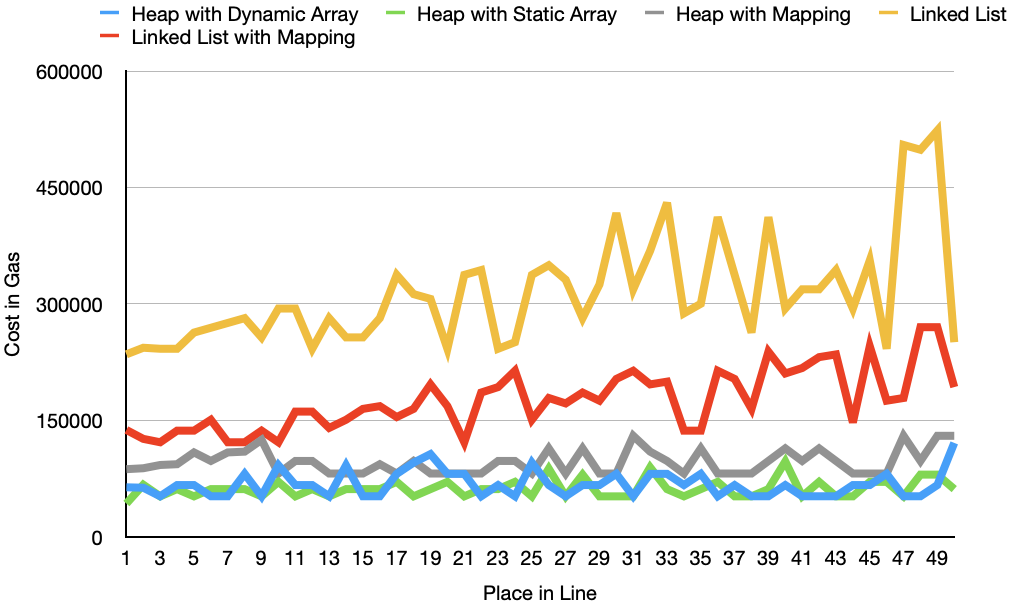
\includegraphics[width=0.8\textwidth]{fig/random_insertion2.png}
\caption{\footnotesize{Gas costs for enqueuing random integers into five priority queue variants. For the x-axis, a value of 10 indicates it is the 10th number entered in the priority queue. The y-axis is the cost of enqueue in gas.}  \label{fig:random_insertion}}
\end{figure}




% = = = = = = = = = = = = = = = = = = = = = = = = = = = = = = = = = = = = = = = =  %

% !TEX root = ../main.tex

% = = = = = = = = = = = =Gas costs and refunds for Dequeueing 50 integers from each PQ  = = = = = = = = = = = = =  %

\begin{table}[t]
\setlength{\tabcolsep}{0.2\tabcolsep}% Shrink \tabcolsep
\centering
\begin{tabular}{|c|c|c|l|}

\multicolumn{1}{c}{} & \headrow{\footnotesize Gas Costs (\texttt{gasUsed})} & \headrow{\footnotesize Refund (Manual)} & \headrow{\footnotesize Full Refund?} \\ \hline

% = = = = = = = = = = = = = = = = = = = = = = = = = = = = = = = = = = = = = = = = = = = = = = = = = = = = = = = = = = = = = = = = = = = = = = %
Heap with Dynamic Array       	& 2,518,131          & 750,000     &\full                  \\ \hline
% = = = = = = = = = = = = = = = = = = = = = = = = = = = = = = = = = = = = = = = = = = = = = = = = = = = = = = = = = = = = = = = = = = = = = = %
Heap with Static Array          	& 1,385,307                             & 750,000      &\full                \\ \hline
% = = = = = = = = = = = = = = = = = = = = = = = = = = = = = = = = = = = = = = = = = = = = = = = = = = = = = = = = = = = = = = = = = = = = = = %
Heap with Mapping 			& 2,781,684                            & 1,500,000    &\full                 \\ \hline
% = = = = = = = = = = = = = = = = = = = = = = = = = = = = = = = = = = = = = = = = = = = = = = = = = = = = = = = = = = = = = = = = = = = = = = %
Linked List                     		& 557,085               	           & 1,200,000      &\full                \\ \hline
% = = = = = = = = = = = = = = = = = = = = = = = = = = = = = = = = = = = = = = = = = = = = = = = = = = = = = = = = = = = = = = = = = = = = = = %
Linked List with Mapping      	& 731,514              	     	  &  3,765,000      &\full                 \\ \hline
% = = = = = = = = = = = = = = = = = = = = = = = = = = = = = = = = = = = = = = = = = = = = = = = = = = = = = = = = = = = = = = = = = = = = = = %

\end{tabular}
\caption{The gas metrics associated with dequeuing 50 integers from five priority queue variants. For the refund, (\full) indicates the  refund was capped at the maximum amount and (\prt) means a greater refund would be possible.
\label{tab:PQUnitTests}}
\end{table}
% = = = = = = = = = = = = = = = = = = = = = = = = = = = = = = = = = = = = =  %


% = = = = = = = = = = = = = = = = = = = = = = = = = = = = = = = = = = = = = = = =  %
%  = = = = = = Table 2 (dequeue) Conversions = = = = = = %
%
%As of July 2020,  $1 gas = 56\times10^{-9} ether$\footnote{https://ethstats.net/} and 1 ether = \$238.33\footnote{https://coinmarketcap.com/}.
%
%$Transaction cost (eth) = GasUsed (unit) \times Gas Price (eth)$ 
%
%%  = = = = = = Transaction Costs in eth = = = = = = %
%
%Heap with Dynamic Array:    		$2,518,131 \times 56\times10^{-9} = 141,015,336\times 10^{-9}$
%Heap with Dynamic Array:     		$1,385,307 \times 56\times10^{-9} = 77,577,192\times 10^{-9}$
%Heap with Mapping:              		$2,781,684 \times 56\times10^{-9} = 155,774,304\times 10^{-9}$
%Linked List:						$557,085 \times 56\times10^{-9} = 	31,196,760\times 10^{-9}$
%Linked List with Mapping:			$731,514 \times 56\times10^{-9} = 	40,964,784\times 10^{-9}$
%
%%  = = = = = = Transaction Costs in USD = = = = = = %
%
%Heap with Dynamic Array:    		$141,015,336\times 10^{-9} \times 238.33 = \$33.60$
%Heap with Dynamic Array:     		$77,577,192\times 10^{-9} \times 238.33 = \$18.48$
%Heap with Mapping:              		$155,774,304\times 10^{-9} \times 238.33 = \$37.12$
%Linked List:						$31,196,760\times 10^{-9} \times 238.33 = \$7.43$
%Linked List with Mapping:			$40,964,784\times 10^{-9} \times 238.33 = \$9.76$
%
% = = = = = = = = = = = = = = = = = = = = = = = = = = = = = = = = = = = = =  %


% = = = = = = = = = = = = = = = = = = = = = = = = = = = = = = = = = = = = = = = =  %


\subsubsection{Dequeue Performance.} For each PQ variant storing 50 random integers, the \texttt{Dequeue()} function is iterated until the data structure is empty. The total gas cost for fully dequeuing the priority queue variants is outlined in Table~\ref{tab:PQUnitTests}. These tests are performed using the following Ethereum gas metrics: block gas limit $=$11,741,495 and 1 gas $=$ 56 Gwei.\footnote{EthStats (July 2020): \url{https://ethstats.net/}} Dequeuing removes data from the contract's storage. Recall this results in a gas refund. Based on our manual estimates (EVM does not expose the refund counter), every variant receives the maximum gas refund possible (\ie half the total cost of the transaction). In other words, each of them actually consumes twice the \texttt{gasUsed} amount in gas before the refund, however none of them are better or worse based on how much of a refund they generate.  

\subsubsection{Discussion.} Based on enqueuing, the heap variants are the cheapest in terms of gas, while based on dequeuing, the link list variants are cheapest. This is in accordance with the theoretical worst-case time complexity for each. However, (i) the linked list variants are materially cheaper than the heap variants at dequeuing, and (ii) dequeuing in a call market must be done as a batch, whereas enqueuing is paid for one at a time by the trader submitting the order, and (iii) Ethereum will not permit more than hundreds of orders so the asymptotic behaviour is not a significant factor. For these reasons, we suggest using a linked list variant for this specific application. As it can be seen in Figure~\ref{fig:random_insertion}, the associated cost for inserting elements into a linked list PQ is significantly greater than the linked list with mapping, as each insertion causes the creation of a new contract. Accordingly, we choose to implement the call market with the linked list with mapping. Overall this PQ balances a moderate gas cost for insertion (\ie order submission) with one for removal (\ie matching the orders). 

% = = = = = = = = = = = = = = = = = = = = = = = = = = = = = = = = = = = = = = = =  %

\subsection{Cost/Benefit of Cleaning up After Yourself}
\label{sec:gasrefund}

% !TEX root = ../main.tex


% = = = = = = = = = = = =Gas costs and refunds for Dequeueing 50 integers from each PQ  = = = = = = = = = = = = =  %

\begin{table}[t]
\centering
\begin{tabular}{|p{7cm}|r|r|r|}

\multicolumn{1}{c}{\.} & \headrow{Gas Costs (\texttt{gasUsed})} & \headrow{Refund (Manual)} & \headrow{Full Refund?} \\ \hline

% = = = = = = = = = = = = = = = = = = = = = = = = = = = = = = = = = = = = = = = = = = = = = = = = = = = = = = = = = = = = = = = = = = = = = = %
% = = = = = = = = = = = = = = = = = = = = = = = = = = = = = = = = = = = = = = = = = = = = = = = = = = = = = = = = = = = = = = = = = = = = = = %
Linked List w/o \texttt{SELFDESTRUCT}         		& 721,370          & 0     &$\times$  \\ \hline
Linked List with \texttt{SELFDESTRUCT}       		& 557,085          & 1,200,000     &\full  \\ \hline
Linked List with Mapping and w/o \texttt{DELETE}    & 334,689          & 765,000     &\full  \\ \hline
Linked List with Mapping and \texttt{DELETE}		& 731,514          & 3,765,000     &\full  \\ \hline

% = = = = = = = = = = = = = = = = = = = = = = = = = = = = = = = = = = = = = = = = = = = = = = = = = = = = = = = = = = = = = = = = = = = = = = %
% = = = = = = = = = = = = = = = = = = = = = = = = = = = = = = = = = = = = = = = = = = = = = = = = = = = = = = = = = = = = = = = = = = = = = = %
% = = = = = = = = = = = = = = = = = = = = = = = = = = = = = = = = = = = = = = = = = = = = = = = = = = = = = = = = = = = = = = = = = = = = = = %

\end{tabular}
\caption{The gas metrics associated with dequeuing 50 numbers from five priority queues variants. For the refund, (\full) indicates the  refund was capped at the maximum amount and \textblue{(\prt) means a greater refund would be possible}.\label{tab:cleaning}}
\end{table}


%  = = = = = = Table 3 (cleaning.tex) Conversions = = = = = = %

%As of July 2020,  $1 gas = 56\times10^{-9} ether$\footnote{https://ethstats.net/} and 1 ether = \$238.33\footnote{https://coinmarketcap.com/}.
%
%$Transaction cost (eth) = GasUsed (unit) \times Gas Price (eth)$ 
%
%%  = = = = = = Transaction Costs in eth = = = = = = %
%
%Linked List with \texttt{SELFDESTRUCT}:     				$557,085 \times 56\times10^{-9} =  31,196,760\times 10^{-9}$  
%Linked List w/o \texttt{SELFDESTRUCT}:     				$721,370 \times 56\times10^{-9} =  40,396,720\times 10^{-9}$ 
%Linked List with Mapping and \texttt{DELETE}:    			$731,514 \times 56\times10^{-9} =  40,964,784\times 10^{-9}$ 
%Linked List with Mapping and w/o \texttt{DELETE}: 		$334,689 \times 56\times10^{-9} =  18,742,584\times 10^{-9}$ 
%
%%  = = = = = = Transaction Costs in USD = = = = = = %
%
%Linked List with \texttt{SELFDESTRUCT}:     				$31,196,760\times 10^{-9}  \times 238.33 = \$7.43$
%Linked List w/o \texttt{SELFDESTRUCT}:     				$40,396,720\times 10^{-9} \times 238.33 = \$9.62$
%Linked List with Mapping and \texttt{DELETE}:    			$40,964,784\times 10^{-9}  \times 238.33 = \$9.76$
%Linked List with Mapping and w/o \texttt{DELETE}: 		$18,742,584\times 10^{-9} \times 238.33 = \$4.46$
% = = = = = = = = = = = = = = = = = = = = = = = = = = = = = = = = = = = = =  %



One consequence of a linked list is that a new contract is created for every node in the list. Beyond being expensive for adding new nodes (a cost that will be bared by the trader in a call market), it also leaves a large footprint on the Ethereum blockchain, especially if we leave the nodes on the blockchain in perpetuity (\ie we just update the head node of the list and leave the previous head `dangling.'). However in a PQ, nodes are only removed from the head of the list; thus the node contracts could be `destroyed' one by one using an extra operation, \texttt{SELFDESTRUCT}, in the \texttt{Dequeue()} function. As shown in Table~\ref{tab:cleaning}, the refund from doing this outweighs to the cost of the extra computation: gas costs are reduced from 721K to 557K.  This suggests a general principle: cleaning up after yourself will pay for itself in gas refunds. Unfortunately, this is not universally true as shown by applying the same principle to the linked list with mapping. 

Dequeuing in a linked list with mapping can be implemented in two ways. The simplest approach is to process a node, update the head pointer, and leave the `removed' node's data behind in the mapping untouched (where it will never be referenced again). Alternatively we can call \texttt{DELETE} on each mapping entry once we are done with a node in the PQ. Deleting a storage variable is identical to setting a non-zero variable to zero (\texttt{SSTORE} 0) that costs 20,000 gas but with 15,000 refunded---a net positive gas cost~\cite{wood2014ethereum}. As it can be seen in the last two rows of Table~\ref{tab:cleaning}, leaving the data on chain is cheaper than cleaning it up.

The lesson here is that gas refunds incentivize developers to clean up storage variables they will not use again, but it is highly contextual as to whether it will pay for itself. Further the cap on the maximum refund means that refunds are not fully received for large cleanup operations (however removing the cap impacts the miners' incentives to include the transaction). This is a complicated and under-explored area of Ethereum in the research literature. For our own work, we strive to be good citizens of Ethereum and clean up to the extent that we can---thus all PQs in Table~\ref{tab:PQUnitTests} implement some clean up and we select linked list with mapping and \texttt{DELETE} for \cm.



% = = = = = = = = = = = = = = = = = = = = = = = = = = = = = = = = = = = = = = = = = =
% = = = = = = = = = = = = = = = = = = = = = = = = = = = = = = = = = = = = = = = = = =
% = = = = = = = = = = = = = = = = = = = = = = = = = = = = = = = = = = = = = = = = = =

\section{Call Market Design}

%GitHub repo:  \footnote{\CallMarketRepo}

% !TEX root = ../main.tex

% = = = = = = = = = = = = = = = = = = = = =Call market operations Table = = = = = = = = = = = =  = = = = = =  %
\begin{table}[t]
\begin{tabular}{|l|l|}
\hline
\multicolumn{1}{|c|}{\textbf{Operation}} & \multicolumn{1}{c|}{\textbf{Description}}                            			\\ \hline

% = = = = = = = = = = = = = = = = = = = = = = = = = = = = = = = = = = = = = = = = = = = = = = = = = = = =  %
	depositToken()                           & Deposits ERC20 standard compliant tokens in \cm smart contract \\ \hline
% = = = = = = = = = = = = = = = = = = = = = = = = = = = = = = = = = = = = = = = = = = = = = = = = = = = =  %
	depositEther()                           	& Deposits ETH in \cm smart contract                        			 \\ \hline
% = = = = = = = = = = = = = = = = = = = = = = = = = = = = = = = = = = = = = = = = = = = = = = = = = = = =  %
	openMarket()                             & Opens the market                                                    					 \\ \hline
% = = = = = = = = = = = = = = = = = = = = = = = = = = = = = = = = = = = = = = = = = = = = = = = = = = = =  %
	closeMarket()                            & Closes the market and processes the orders       \\ \hline
% = = = = = = = = = = = = = = = = = = = = = = = = = = = = = = = = = = = = = = = = = = = = = = = = = = = =  %
	submitBid()                              & Inserts the upcoming bid order messages inside the priority queue    \\ \hline
% = = = = = = = = = = = = = = = = = = = = = = = = = = = = = = = = = = = = = = = = = = = = = = = = = = = =  %
	submitAsk()                              & Inserts the upcoming ask order messages inside the priority queue    \\ \hline
% = = = = = = = = = = = = = = = = = = = = = = = = = = = = = = = = = = = = = = = = = = = = = = = = = = = =  %
	claimTokens()                           & Transfers tokens to the traders                       			\\ \hline
% = = = = = = = = = = = = = = = = = = = = = = = = = = = = = = = = = = = = = = = = = = = = = = = = = = = =  %
	claimEther()                             & Transfers ETH to the traders                       			\\ \hline
% = = = = = = = = = = = = = = = = = = = = = = = = = = = = = = = = = = = = = = = = = = = = = = = = = = = =  %
\end{tabular}
\caption{\footnotesize{Primary operations of \cm smart contract.}
\label{tab:cm_functions}}
\end{table}

% = = = = = = = = = = = = = = = = = = = = = = = = = = = = = = = = = = = = = = = = = = = = = = = = = = = =  %

\cm is intended as a module that developers can modify as they choose---thus we tried to simplify the design at every step to make it highly extensible but still functional without any extensions. A call market will open for a specified period of time during which it will accept orders. Orders are added to a PQ. Our vision (discussed below) is the market would be open for a very short period of time, close, and then reopen immediately (\eg every other block). We keep the design simple by not allowing cancellations. Because markets are relatively short-lived, cancelations require a second transaction, and front-running attacks apply to cancellation orders~\cite{eskandari2019sok}, orders simply expire when the market call period ends. 

Another simplifying assumption was to implement a \textit{collateralized} call market. We assume all trades are between ETH and an ERC20 token, all orders are pre-funded in the contract with ETH (for bids) and tokens (for asks), and once ETH or tokens are committed to an order, they cannot be withdrawn until the market closes. This ensures all executed orders clear and settle (\ie no defaults on payment or delivery).

% Volume of 1
% Ties?

\cm is written in 324 lines (SLOC) of Solidity,~\footnote{Github: linked removed for anonymity} a high level programming language that is syntactically similar to Java~\cite{Ethereum41:online}. We tested it with the Mocha testing framework (tests included in the codebase), as deployed using Truffle on Ganache-CLI to obtain our performance metrics. Table~\ref{tab:cm_functions} represents \cm's primary operations.

%============= Performance =================== %

 \subsection{Measurements}
 
 % !TEX root = ../main.tex

\begin{table}[t]
\setlength{\tabcolsep}{0.1\tabcolsep}% Shrink \tabcolsep
\centering
\begin{tabular}{|l|r|r|r|r|}

\multicolumn{1}{c}{} & 

\headrow{Max trades (w.c.)} & 
\headrow{Gas for max trades} & 
\headrow{Gas for 1000 trades} & 
\headrow{Gas for order (avg)} \\ \hline

% = = = = = = = = = = = = = = = = = = = = = = = = = = = = = = = = = = = = = = = = = = = = = = = = = = = = = = = = = = = = = = = = = = = = = = %
Heap with Dynamic Array       & 38            & 5,372,679                   	& 457,326,935      & 207,932     \\ \hline
% = = = = = = = = = = = = = = = = = = = = = = = = = = = = = = = = = = = = = = = = = = = = = = = = = = = = = = = = = = = = = = = = = = = = = = = = = = = = = = = = = %
Heap with Static Array          	& 42            & 5,247,636                  	& 333,656,805         & 197,710         \\ \hline
% = = = = = = = = = = = = = = = = = = = = = = = = = = = = = = = = = = = = = = = = = = = = = = = = = = = = = = = = = = = = = = = = = = = = = = = = = = = = = = = = = %
Heap with Mapping 		& 46           	 & 5,285,275                     & 226,499,722    & 215,040           \\ \hline
% = = = = = = = = = = = = = = = = = = = = = = = = = = = = = = = = = = = = = = = = = = = = = = = = = = = = = = = = = = = = = = = = = = = = = = = = = = = = = = = = = %
Linked List                     	& 152            & 5,495,265                     & 35,823,601         & 735,243             \\ \hline
% = = = = = = = = = = = = = = = = = = = = = = = = = = = = = = = = = = = = = = = = = = = = = = = = = = = = = = = = = = = = = = = = = = = = = = = = = = = = = = = = = %
Linked List with Mapping      	& 86             & 5,433,259                     & 62,774,170        &  547,466              \\ \hline
% = = = = = = = = = = = = = = = = = = = = = = = = = = = = = = = = = = = = = = = = = = = = = = = = = = = = = = = = = = = = = = = = = = = = = = = = = = = = = = = = = %

\end{tabular}
\caption{\footnotesize{Performance of \cm for each PQ variant \textblue{Reviewer's comment:  Gas for max trades in table 5 is about 5M gas, why it can exceed 11M gas limit of Ethereum?}}.\label{tab:worst_case_matching}}

\end{table}
% = = = = = = = = = = = = = = = = = = = = = = = = = = = = = = = = = = = = =  %





 
The main research question is how many orders can be processed in a single Ethereum transaction when the closing the call market, using Ethereum today. As our previous experiments indicated, the choice of priority queue (PQ) implementation is the main influence on performance (see Table~\ref{tab:worst_case_matching}). We implemented a generic call market that interfaces with a generic PQ (at its own contract address) and ran experiments for each PQ implementation. We looked at the \textit{worst-case} for performance which is when every submitted bid and ask is marketable (\ie will require fulfillment). In the first two columns, we determined the highest number of orders that can be processed in a single call to the \texttt{closeMarket()} and not exceed the the current Ethereum block gas limit of 11,741,495. Since Ethereum will become more efficient over time, we also were interested in how much gas it would cost to execute 1000 pairs of orders which is given in the third column. The fourth column indicates the cost to the trader of submitting a bid or ask --- since this costs will vary depending on how many orders are already submitted (recall Figure~\ref{fig:random_insertion}), we average the cost of 200 order submissions. 

As expected, the numbers closely track the performance of the PQ itself suggesting the PQ is indeed the main influence on performance. In Ethereum today, call markets appear to be limited to processing about a hundred orders per transaction. If markets open on every other block and the call market could monopolize an entire block to close, a few hundred orders per minute (worst-case) can be processed. The main takeaway is that the transparency, front-running resistance, and low barrier to entry of Ethereum comes with an enormous cost (\ie an institutional exchange like NASDAQ can process 100K trades per second). That said, many exchanges trade the same assets under different trading rules (\ie market fragmentation) because traders have different preferences. \cm can work today in some circumstances like very low liquidity tokens, or markets with high volumes and a small number of traders (\eg liquidation auctions). 

\subsection{Security Analysis} \label{sec:front}

\paragraph{Code Security.} We used two security audit tools, \textit{Slither}\footnote{https://github.com/crytic/slither} and \textit{SmartCheck},\footnote{https://tool.smartdec.net} on \cm to find vulnerabilities and bad practices across 67 tests. \cm passes all test except some `informational' warnings (\eg a costly loop) that are intentional design choices.

\paragraph{Front-running.} The primary motivation for using a call market, as opposed to a continuous time order book, is to mitigate front-running attacks~\cite{clark2014decentralizing,eskandari2019sok,daian2019flash}. Consider a sequence of 100 orders submitted within a window of time to market A, and the same sequence is randomly shuffled and submitted to market B. If A and B are continuous, the orders that are executed in A could be quite different from B. In a call market, the outcome of A and B will be exactly equivalent. There is no threat from miners reordering transactions or traders offering higher gas rates to have their orders executed before other orders already broadcasted. 

Potential for front-running still exists around ties on price and cancelations (see below). Finally, \textit{displacement attacks}~\cite{eskandari2019sok} are possible where competitive orders are delayed long enough for the market to close without them. In a traditional call market, a market clearing price is chosen and all trades are executed at this price. All bids made at a higher price will receive the assets for the lower clearing price (and conversely for lower ask prices): this is called a price improvement. A miner about to mine on a set of transactions, including its own orders, could drop other traders' orders to maximize its own price improvement. For this reason, in \cm, all price improvements are given to the miner (using \texttt{block.coinbase.transfer()}). This does not actively hurt traders---they always receive the same price from their order---and it removes any incentive to front-run these profits. For all these reasons, we say \cm reduces front-running attacks but stop short of saying it is completely solved by \cm. 

% = = = = = = = = = = = = = = = = = = = = = = = = =  %

\section{Design alternatives and extensions}

As a module, we try to keep \cm as simple as possible, and allow customization and extensions as appropriate. We discuss potential modifications here.  

\subsection{Token Divisibility and Volumes} 

We implement a very simple market where orders all have the same volume: 1 token. Traders submit multiple orders to increase volume. To extend orders with a volume field, it must first be determined if the token are non-divisible or divisible (and to what precision). In this case, \texttt{closeMarket()} needs to look at multiple bids to fulfill a single ask (and vice-versa) and declare its trading rules on partial fills. We also simplify the market rules around ties on price: we execute them FIFO (breaking front-running resistance for ties on prices). A common trading rule (that does resist front-running) is to fill ties in proportion to their volume (\ie \textit{pro rata} allocation)\footnote{If Alice and Bob bid the same price for 100 tokens and 20 tokens respectively, and there are only 60 tokens left in marketable asks, Alice receives 50 and Bob 10.} however this approach is also contingent on the divisibility of tokens. Consider the following corner-case: 3 equally priced bids of 1 non-divisible token and 1 ask at the same price. There is not good option: (1) the bids could all be dropped (fair but not market efficient), (2) bids could be prioritized based on time as in \cm (front-running is viable, but in this corner case only), or (3) the bid could be randomly chosen (\cf Libra~\cite{mavroudis2019libra}); blockchain `randomness' is generally deterministic and manipulatable by miners~\cite{bonneau2015random,buenz2017proofs} and counter-measures could take a few blocks to select~\cite{boneh2018verifiable}).

\subsection{Cancelations}

\cm does not support trade cancelations. We intend to open and close markets quickly (on the order of blocks), so orders are relatively short-lived. Support for cancelation also opens the market to new front-running issues where other traders (or miners) can displace cancelations until after the market closes (however one benefit of a call market is that beating a cancelation with a new order has no effect, assuming the cancelation is run any time before the market closes). Finally, cancelations have a performance impact. Canceled orders can be removed from the underlying data structure   or accumulated in a list that is cross-checked when closing the market. Removing orders requires a more verbose structure than a priority queue (\eg a binary search tree instead of a heap; or methods to traverse a linked list rather than only pulling from the head). While client software could help point out where the trade is in the data structure, the orderbook can change between submitting the cancelation request and running the method. A linked list with mapping that returns the key for each submitted order seems to be the most tenable data structure. 

\subsection{Market clearing price}

Call markets are heralded for fair price discovery. This is why many exchanges use a call market at the end of the day to determine the closing price of an asset, which is an important price both optically (it is well-published) and operationally (many derivates settle based on the closing price). We purposely do not compute a `market clearing price' with \cm because miners can easily manipulate the price (\ie include a single wash trade at the price they want fixed), although they forgo profit for doing so. This is not merely hypothetical---Uniswap (the prominant quote-drive, on-chain exchange) prices have been manipulated to exploit other DeFi applications relying on them. Countermeasures to protect Uniswap price integrity could also apply to \cm: (1) taking a rolling mediant of prices over time, and (2) using it alongside other sources for the same price and forming a consensus. While \cm does not emit a market clearing price, it can be computed by a webapp examining the orderbook at market close. 

\subsection{Scheduling events}

As a simple module, \cm is a one-shot market. However it can be extended to re-open with a clean orderbook after \texttt{closeMarket()} is run. Modifiers can enforce when the market operates openly (collecting orders) and when close can be run. In the Princeton paper~\cite{clark2014decentralizing}, the call market is envisioned to run as an alt-coin, where orders accumulate within a block and a miner closes the market as part of the logic of producing a new block (\ie within the same portion of code as computing their coinbase transaction in Bitcoin or Gas Used in Ethereum). 

If the call market runs as a DApp on Ethereum, it seems difficult to open and close the market every block. Someone needs to call \texttt{closeMarket()} for every block (we return to who this is next) but the market will only work as intended if miners execute this function after every \texttt{submitBid()} and \texttt{submitAsk()} invocation. Since price improvements are paid to the miners, the miner is incentivized to run \texttt{closeMarket()} last to make the most profit. Perhaps in a world where these markets became immensely popular, miners would actually do this, but as it stands, miners do not generally search for the transaction ordering that nets them the most profit.

A close alternative is to allow markets to open and close on different blocks. Specifically, the \texttt{closeMarket()} function calls \texttt{openMarket()} as a subroutine and sets two modifiers: orders are only accepted in the block immediately after the current block (\ie the block that executes \texttt{closeMarket()}) and \texttt{closeMarket()} cannot be run again until two blocks after the current block. 

The final issue is who invokes \texttt{closeMarket()} every other block? There are actually two issues here: the issue of scheduling the function call and the issue of paying for it. For scheduling the function call, we can do one of the following: rely on market participants who are eager to trade to reopen the market, offer a bounty to reopen the market, or use an external service like Ethereum Alarm Clock.\footnote{\url{https://ethereum-alarm-clock-service.readthedocs.io/}} Next we consider the second issue of who pays to close the market. 

% = = = = = = = = = = = =Who Pays the Cost for Closing and Reopening the Market?= = = = = = = = = = = = =  %

\subsection{Who pays to close/reopen the market?}

It is unlikely that a mining software will become aware of specific DApps, but miners are paid all price improvements in the market and so it is possible that running \texttt{closeMarket()} would pay for itself. However we consider two other (more realistic) scenarios. One solution requires a modified closing function, \texttt{closeMarket(n)}, that only processes $n$ orders at a time (until the order book is empty). Once the time window for submitting orders is past, a new market is created (without settling the previous market). Every orders to the new market is also requires to run, say, \texttt{closeMarket(10)} on the older market, thus progressively closing the previous market while accepting orders to the new market. This solution pattern has two issues: first, amortizing the cost of closing the market amongst the early traders of the new market is an added incentive to not submit orders early to the market; the second related issue is if not enough traders submit orders in the new market, the old market never closes (resulting in a backlog of old markets waiting to close).

The second solution is to levy a carefully computed fee against the traders for every new order they submit. The fees are accumulated by the DApp to use as a bounty. When the time window for the open market elapses, the user who calls \texttt{closeMarket()} receives the bounty. This is a better solution, although not perfect: \texttt{closeMarket()} cost does not follow a tight linear increase with the number of orders, and gas prices vary over time which could render the bounty insufficient for offsetting the \texttt{closeMarket()} cost. However an interest third party (such as the token issuer for a given market) might bailout the market when it halts on \texttt{closeMarket()} to facilitate further trading. If the contract can pay for its own functions, an interested party can also arrange for a commercial service (\eg any.sender\footnote{\url{https://github.com/PISAresearch/docs.any.sender}}) to relay the \texttt{closeMarket()} function call on Ethereum (an approach called \textit{meta-transactions}). 

%= = = = = =  = =  =  Rollups=  = = = = = = = = =%

\subsection{Off-chain closing}
\label{sec:rollups}

We have two main motivations for designing an \textit{on-chain} order book: (1) the trust model is superior to partially/fully centralized solutions, and (2) \cm can be deployed without any delay or other arrangements. We have relaxed (2) already by considering services like Ethereum Alarm Clock and any.sender to facilitate easy market closings. In this section, we present a variant that only provides (1) (however one that can be deployed without any other market stakeholders). 

A function can be computed off-chain and the new state of the DApp, called a \textit{rollup}, is written back to the blockchain, accompanied by either (1) a proof that the function was executed correctly, or (2) a dispute resolution process that can resolve, on-chain, functions that are not executed correctly (\eg Arbitrum~\cite{kalodner2018arbitrum}). In the case of (1), validating the proof must be cheaper than running the function itself. There are two main approaches to (1): the first is to use cryptographic proof techniques (\eg SNARKS~\cite{BCGTV13,GGPR13} and variants~\cite{BBHR19}), and the second is to execute the function in a trusted execution environment (TEE; \eg Intel SGX) and validate the TEE's quote on-chain (\eg Ekiden~\cite{cheng2019ekiden}).\footnote{The TEE-based approach is mired by recent attacks on SGX~\cite{SGX1,SGX2,SGX3,SGX4}, however these attacks do not necessarily apply to the specifics of how SGX is used here, and safer TEE technologies like Intel TXT (\cf~\cite{ZBC+19}) can be substituted.}

We implement a variant of \cm using rollups on Arbitrum.\footnote{\url{https://offchainlabs.com} for more current details than the 2018 \textit{USENIX Security} paper~\cite{kalodner2018arbitrum}.} In this model, the token issuer (or other interested party) will run a dedicated server to watch Ethereum for function invocations submitted and sequenced on-chain, perform the function call off-chain, and write the resultant state on-chain. Anyone capable of running EVM code can verify the result. If it is incorrect, a dispute can be filed (with the correct state) and an on-chain correction will be made. With or without disputes, participants that validate the function calls for themselves can proceed knowing that the correct state will eventually be finalized. 

In our \cm variant with rollups, the token issuer is does all the computation (both enqueuing and dequeuing). Thus we switch the priority queue to use a heap with dynamic array, which balances the expense of both operations (instead of optimizing for dequeuing in \texttt{closeMarket()}). Recall that on-chain, such a priory queue can only match 38 pairs at a cost of 5,372,679 gas. With roll-ups, 38 pairs cost 38,863 gas. As the pairs increase, the cost is essentially constant (\eg 1000 pairs cost 38,851 as opposed to 457,326,935 on-chain). Submitting an order costs 39,169 gas on average as opposed to 207,932 on-chain.

Our \cm variant is not the first rollup-based order book. Loopring 3.0\footnote{\url{https://loopring.org}} offers a continuous time order book. The primary difference is that orders in Loopring 3.0 are submitted off-chain to the operator directly, whereas our variant requires on-chain submission. While on-chain submission is hampered by Ethereum's block limits, the threat model of reordering transactions is well-understood and our call market design mitigates most front-running attacks. In Loopring 3.0, the rollup proof does not ensure that the exchange did not reorder transactions, which is particularly problematic in a continuous time order book. In short, we provide better protection against a malicious exchange while Loopring 3.0 provides even better performance.


%% = = = = = = = = = = = =Transferring the Collateral back to the traders = = = = = = = = = = = = =  %
%\subsection{Collateralization}
%
%Options for non-collateralized markets
%ERC20 to ERC20 -> extra transaction
%



% = = = = = = = = = = = = = = = = = = = = = = = = = = = = = = = = = = = = = = = = = =

\section{Concluding Remarks} 

Imagine you have just launched an ERC20 token on Ethereum. Now want your holders to be able to trade it. While the barrier to entry for exchange services is low, it still exists. For a centralized or decentralized exchange, you have to convince the operators to list your token and you will be delayed while they process your request. For an automated market maker, you will have to lock up a large amount of ETH into the DApp, along with your tokens. For rollups, you will have to host your own servers or list it with an exchange. By contrast to all of these, with \cm you just deploy the code alongside your token and trading is immediately supported. Even if \cm is a fallback solution today, we believe it is helpful for every token to be accompanied by on-chain trade execution. With future improvements to blockchain scalability, it could become the defacto trading method.
 
%\subsubsection*{Acknowledgements.} J. Clark thanks ...































